\section{MARAKA PLANETS – PLANETS THAT CAN CAUSE DEATH AND INJURY}
 

This lesson will provide advanced material for Part II of the course relative to medical astrology and should be viewed in that context.

 

We have mentioned Maraka planets briefly already. Here we will focus on them in some detail.

 

Maraka (literally death-causing) planets are first of all planets that rule houses 2 and 7 from the Ascendant. Secondly they are planets located in these houses. As these houses are twelfth from the houses of life and longevity, 3 and 8, they gain the power to negate them or bring their influences to an end. Planets in houses 2 and 12 from the Moon gain a Maraka status to some degree as well. Natural Maraka or destruction-bringing planets are Saturn and Ketu, and by some accounts Mars. If these are also temporal Marakas in the chart their influence is yet more powerful.

 

However the term Maraka should not be taken too literally. Such planets do not always bring death. Sometimes they bring some risk of death, or only ill health or injury. If there are no strong afflictions in the chart they may do nothing at all.

 

They may simply bring their usual results, like the seventh lord bringing marriage. Yet if the chart is afflicted or if the person is elderly the periods of such Maraka planets can cause health problems or even death. We have already introduced them relative to medical astrology. Here we will examine them in more detail.

 

I realize that this subject can be a little morbid, perhaps only appealing to Saturnian types, but it can help us with difficult situations and, we must remember, people are always more likely to come to us with their difficulties. If such negative influences are not found to be active in the chart this itself is an important sign of positive good fortune. If they are found then noting them can give the client some room for either avoiding their influences or preparing for it.

 

\subsection{Referred Houses}
 

We will use this issue of Marakas to make a second point, to show how referred houses can be read both as to their inherent strength and relative to the Dashas.

 

It is possible to read in the birthchart the condition not only of the native, but also of his relations. This is done through referred houses, the fourth for the mother, the ninth for the father and so forth.
 

The health and longevity of these people in our lives can be read from such houses as well. The main way of reading the life of our relatives is by turning the house relating to them into the Ascendant and reading positions from there. The status of their natural significator, like the Moon for the mother, must be borne in mind as well.

 

We can consider these referred houses in the Dasha scheme as well.
 

For example, if a Capricorn ascendant person is running a Mars period, as Mars is the fourth lord it would have some impact upon the Mother. Regarding Aries as the Ascendant for the mother, which is the case then, if the native is running the period of Jupiter, not a benefic for the native but for the mother, one could expect some benefit to the mother. Similarly if the native is running a period of Saturn, the Ascendant lord, this could have negative consequences for the mother because Saturn is a bad planet for Aries.

 

Maraka rules, like the other rules of Vedic Astrology, also function from referred houses. For example, relative to the fourth house of the mother, malefics in the tenth house, which is seventh from the fourth, can cause her harm. Dashas of malefic lords from the fourth house can harm the Mother as well. On the other hand, benefics in such positions will benefit her.

 

Most of us astrologers and most of the people who come to us are middle aged, between 35 and 50. This means that our parents will be over 60. As all Maraka planets gain potency after the age of 65 even in a good chart, it is clear that most of our parents will be in a position where Maraka influences can come into play.

 

Therefore examining the chart of a person over forty years old relative to the fourth and ninth houses can be an important way of determining the longevity of their parents In fact the death of the parents is often more clear from the charts of their children than their own. Such cross-referencing of charts can help us provide more accurate interpretations. Taking the charts of family members and then reading the same influences in referred houses in the individual charts is a good tool for learning Vedic Astrology.

 

\subsection{Example Charts}
\subsubsection{Chart 1}

 
\begin{figure}[h]
\centering
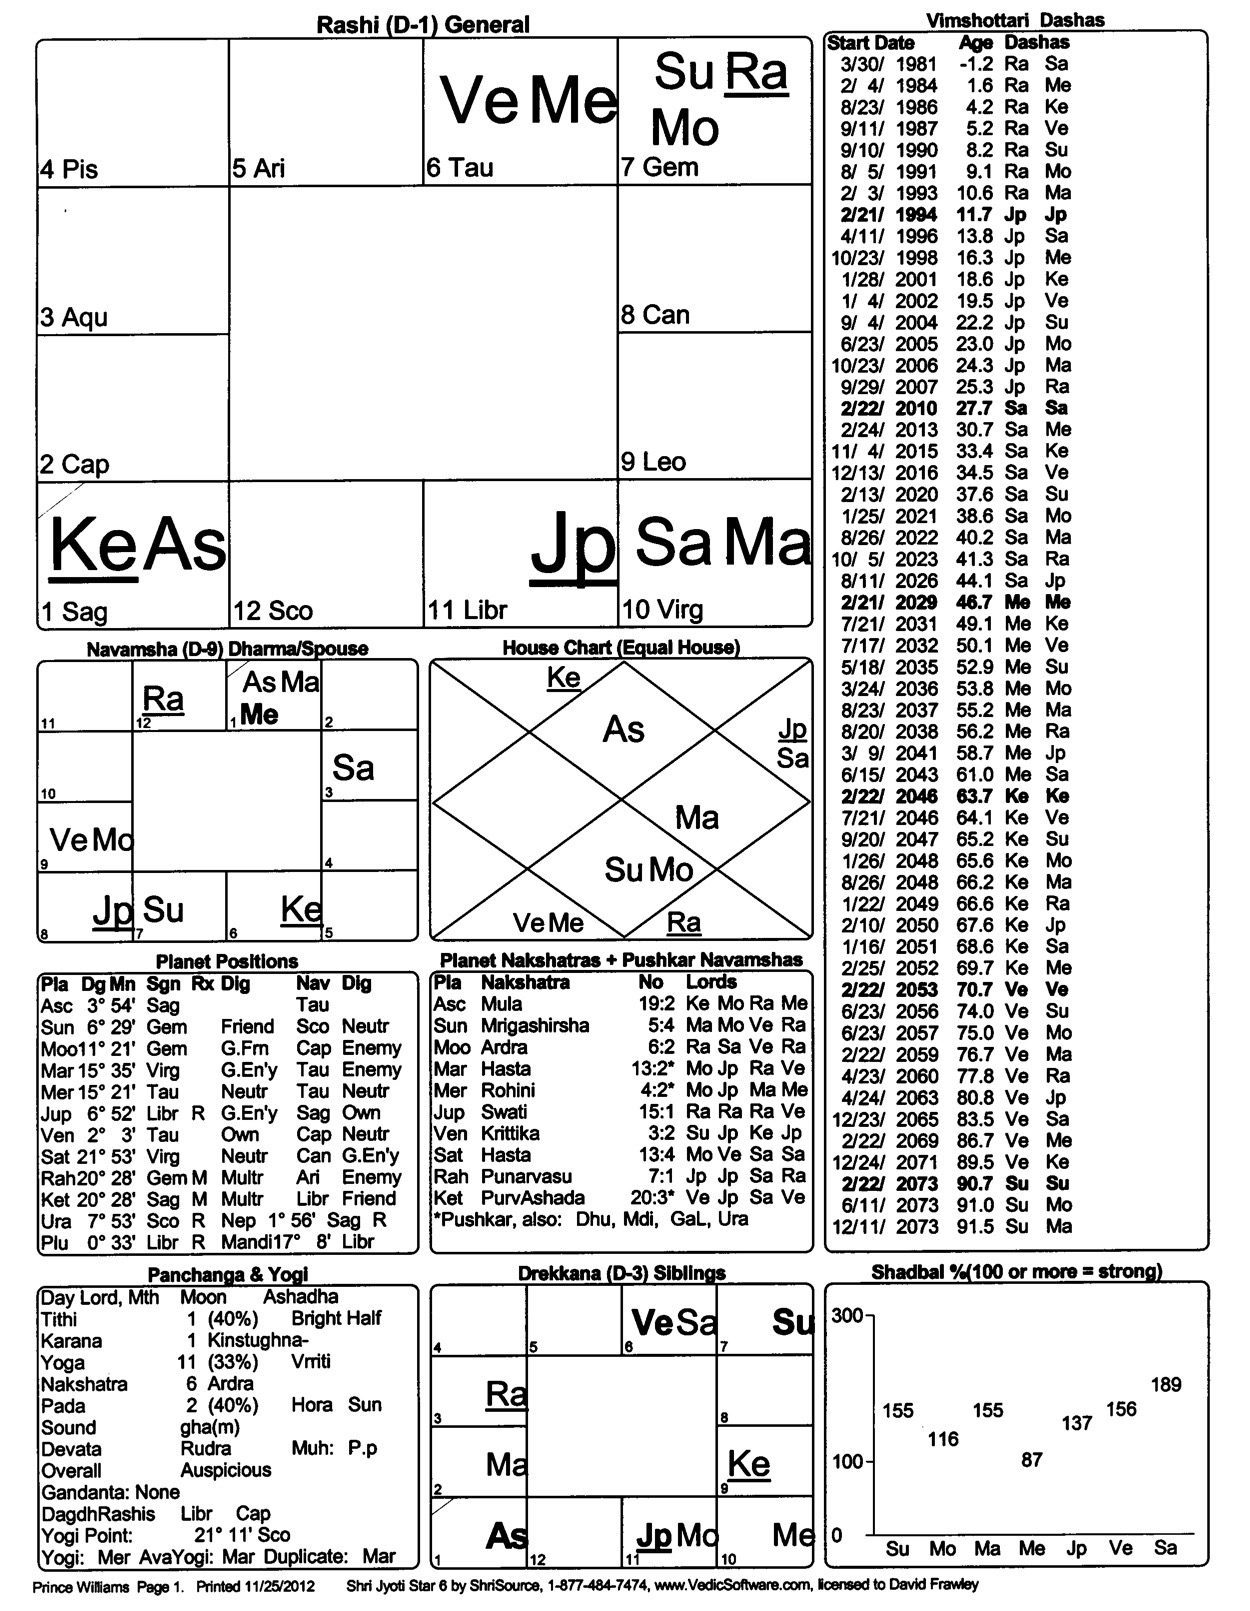
\includegraphics[width=10cm]{pics/Lesson6chart1.jpg}
\caption{}
\end{figure}

The death of parents is often obvious in the charts of their children, particularly if the parents die young. The reason for this is that the early death colors the entire life of the child very strongly.

 

Here we will use the chart of Prince William, the eldest son of Princess Diana, who recently died in a car crash. Such a tragic event should be indicated in the chart of the child. William has a Sagittarius Ascendant along with Ketu. Mercury and Venus are together in the sixth house. Sun, Moon and Rahu are in Gemini in the seventh house. Mars and Saturn are in Virgo in the tenth house. Jupiter is retrograde in Libra in the eleventh house. His mother died during Jupiter Dasha Saturn Bhukti.

 



 

Taking the fourth house, Pisces, to be the Ascendant, Jupiter is the lord of Lagna. It is located retrograde in Libra in the eighth house from Pisces, a house of death. Mars and Saturn, two strong malefics are in the Virgo, seventh from and aspecting the Lagna of the mother. Saturn is also a temporal malefic for Pisces ruling the eleventh and twelfth from it. Mars is a benefic for Pisces but is tainted by ruling the second house and thereby becomes a Maraka. Both planets are located in a Maraka house, the seventh, from the Lagna of the mother.

 

In addition Saturn aspects the Moon, the significator of the Mother with its tenth aspect. The Moon itself is new and combust the Sun, just five degrees past an eclipse of the Sun, and with Rahu. It is in Ardra a cruel Nakshatra ruled by Rahu. Furthermore the Moon is in a Maraka house from the Ascendant and is itself the lord of the eighth. Mars and Saturn are also located in the fourth house (Virgo) from the Moon (in Gemini) strongly afflicting it. Therefore all the factors of the mother are highly afflicted.

 

Looking at the Navamsha position, Mars a great malefic for Taurus Ascendant aspects both the fourth house, Leo in the Navamsha, and its lord the Sun. The Moon is in a sign of Saturn aspected by Saturn. The Moon is the seventh from its own sign in Capricorn and Saturn, the second from the Moon, is located in the seventh from it. So Navamsha positions are also afflicted.

 

The mothers death occurred in the combined periods of Jupiter-Saturn-Rahu. Jupiter, the lord of the Mothers house, is highly afflicted and so shows important events relative to her that are not likely to be good. Saturn is in a maraka house from the house of the mother and a natural malefic for it. It afflicts the Moon in the birthchart as does Rahu. In the Navamsha Saturn also aspects the Moon, Jupiter is the eighth lord from the house of the mother, and Rahu is located in the eighth house from the house of the mother.

 

\subsubsection{More on Referred Houses}

 

Note that the afflictions to the fourth house from the house of the mother in the birthchart show the emotional turbulence in the mothers life. The afflictions to the seventh house from the mothers Lagna, the fourth house, show the marriage and partnership problems in her life. Taking this principle further whenever a house has many planets in it, is highly afflicted or very auspicious, we can also see how it is affecting the referred houses in the chart and which relations of the native are involved with it. This use of referred houses gives us a more multidimensional astrology and a multisided approach to the chart.

 

In this regard let us take a quick look at the same chart relative to the father. Leo as the ninth house becomes the Ascendant for the father. The Sun, the lord of the Ascendant, is also the natural significator for the father. The birth occurred shortly after a solar eclipse and the Sun is with the Moon and Rahu. The Moon and Rahu dominate the chart of the father, Prince Charles, as noted under his chart as an example for Cancer Ascendant. These planets are located in the eleventh house for the father (eleventh from the ninth in the birthchart), a strong position but a compromised combination. The aspect of Saturn further compromises them.

 

Mercury and Venus are together in Taurus in the tenth house for the father, a Maha Purusha Yoga for Venus and a Dhana Yoga as Mercury is the second and eleventh lord. The second house for the father, that of expression is afflicted by Mercury and Saturn. The Lagna is free of any affliction by Marakas, which for Leo are Mars and Saturn. Saturn afflicts the Lagna lord. Jupiter is not a Maraka for the father in the chart as it is for the Mother. The Saturn period for Prince William does not begin until 2010, so his chart does not appear to show such affliction to the father as to the mother.

 

Hence we can determine the health of other relatives in the chart as to the influences on their respective houses and house lords: the third for younger siblings, the fourth for the mother, the fifth for children, the seventh for the spouse, the ninth for the father, and so on.

 

\subsubsection{Chart 2}


 \begin{figure}[h]
\centering
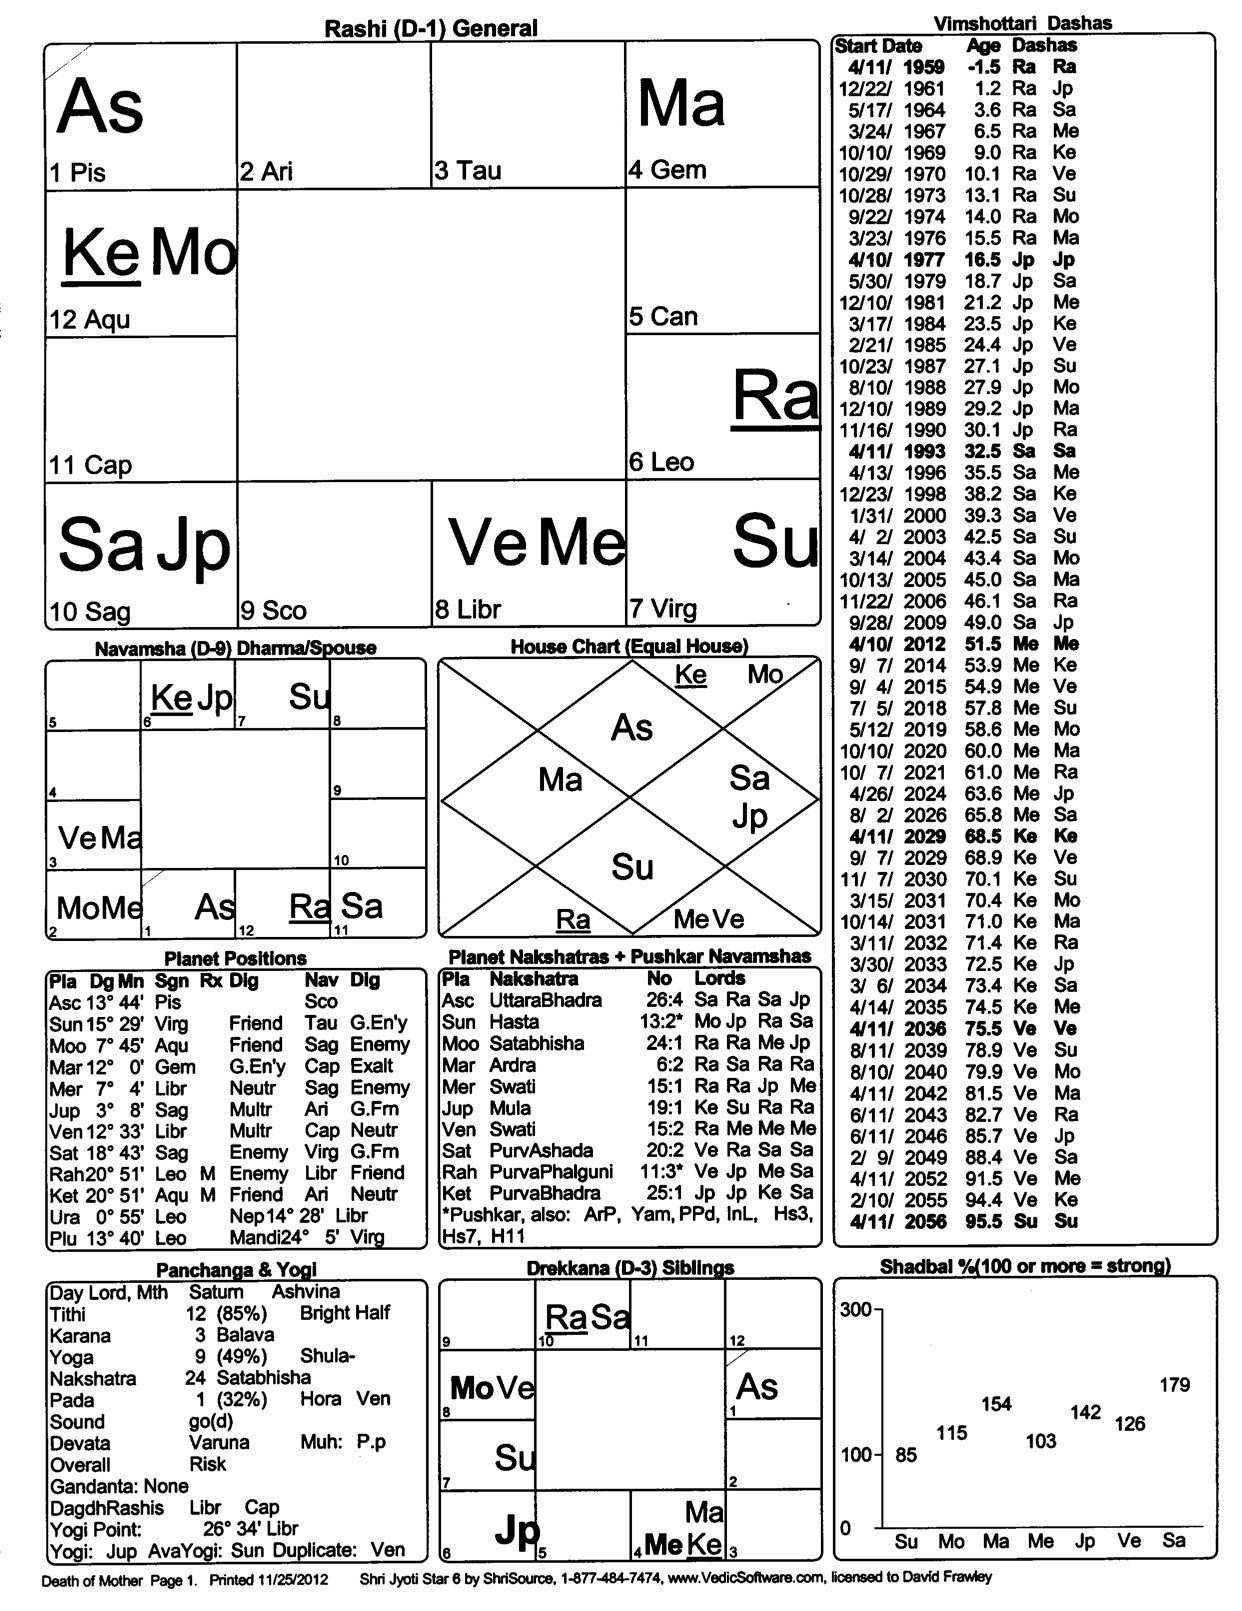
\includegraphics[width=10cm]{pics/Lesson6chart2.jpg}
\caption{}
\end{figure}

This chart has a similar orientation as the previous chart in that the fourth house and the Moon are highly afflicted. The natives mother died in April 1981 under Jupiter-Saturn from a congenital heart defect that surgery failed to correct.

 

The Ascendant is Pisces and so the fourth house is Gemini. Turning that house into the Ascendant for the mother we can read the chart from there. Gemini contains

 



 

Mars, the worst planet for Gemini. It is also aspected by Saturn, the eighth lord, and Jupiter, the seventh lord, a Maraka planet from a Maraka house. Mercury, lord of the fourth house, is in the difficult eighth house from the Lagna along with Venus, the eighth lord. The Moon itself is in the difficult twelfth house from the Ascendant aspected by Saturn and in the same sign with Ketu. With such strong afflictions on need not look much further before considering that the mothers fate is very difficult Relative to the Dashas, Jupiter-Saturn would project the afflictions inherent in their positions.

 

Of course other features of the chart are there as well. The Moon-Ketu combination in the twelfth, with the Moon as fifth lord, makes the native highly spiritual but psychically sensitive and vulnerable. The affliction of the Moon as fifth lord, the fifth house being hemmed in by malefics Mars and Rahu, and Mars in the fifth from the Moon denies the woman children. Saturn and Mars aspecting the Sun in the seventh house denies her marriage. Mercury and Venus in the eighth are additional spiritualizing influences and also give her a good inheritance.

 

Similar afflictions prevail in the Navamsha with the Sun in the seventh, and Mars aspecting the fifth lord in the sixth house with Ketu. Hence once we have gained access into a chart we can begin seeing its patterns in many ways and its ramifications in all areas of the persons life and relationships.

 

\subsubsection{Caution to the Astrologer}

 

Naturally this type of examination of maraka houses can be both fascinating and frightening. We have to be careful about predicting dramatic consequences for the future until we have really gone into a chart thoroughly. Ways to do this include examining the charts of a persons relatives and examining the natives yearly charts (varshaphal) as well. Another method is to correlate their personal history with the respective planetary periods and use this to gauge the effect of the planets operating in those periods.

 

Finally one must remain humble. Astrology can show difficulty or ease but determining ahead of time whether a particular difficult planetary period will bring general obstacles, health problems, or trouble to a particular relationship of the native is not always easy. Similarly a good planetary period may bring only one type of benefit or it may bring benefit on several levels. Beyond this timing specific events by prediction is yet more difficult.

 

Here we see the advantage of maintaining a long-term relationship with clients. It can take some time and interchange before the secrets of a persons chart begin to become clear to the astrologer. One should not expect this after a causal glance or a single reading.

 

\subsubsection{Chart 3:
A Chart of Great Longevity}


\begin{figure}[h]
\centering
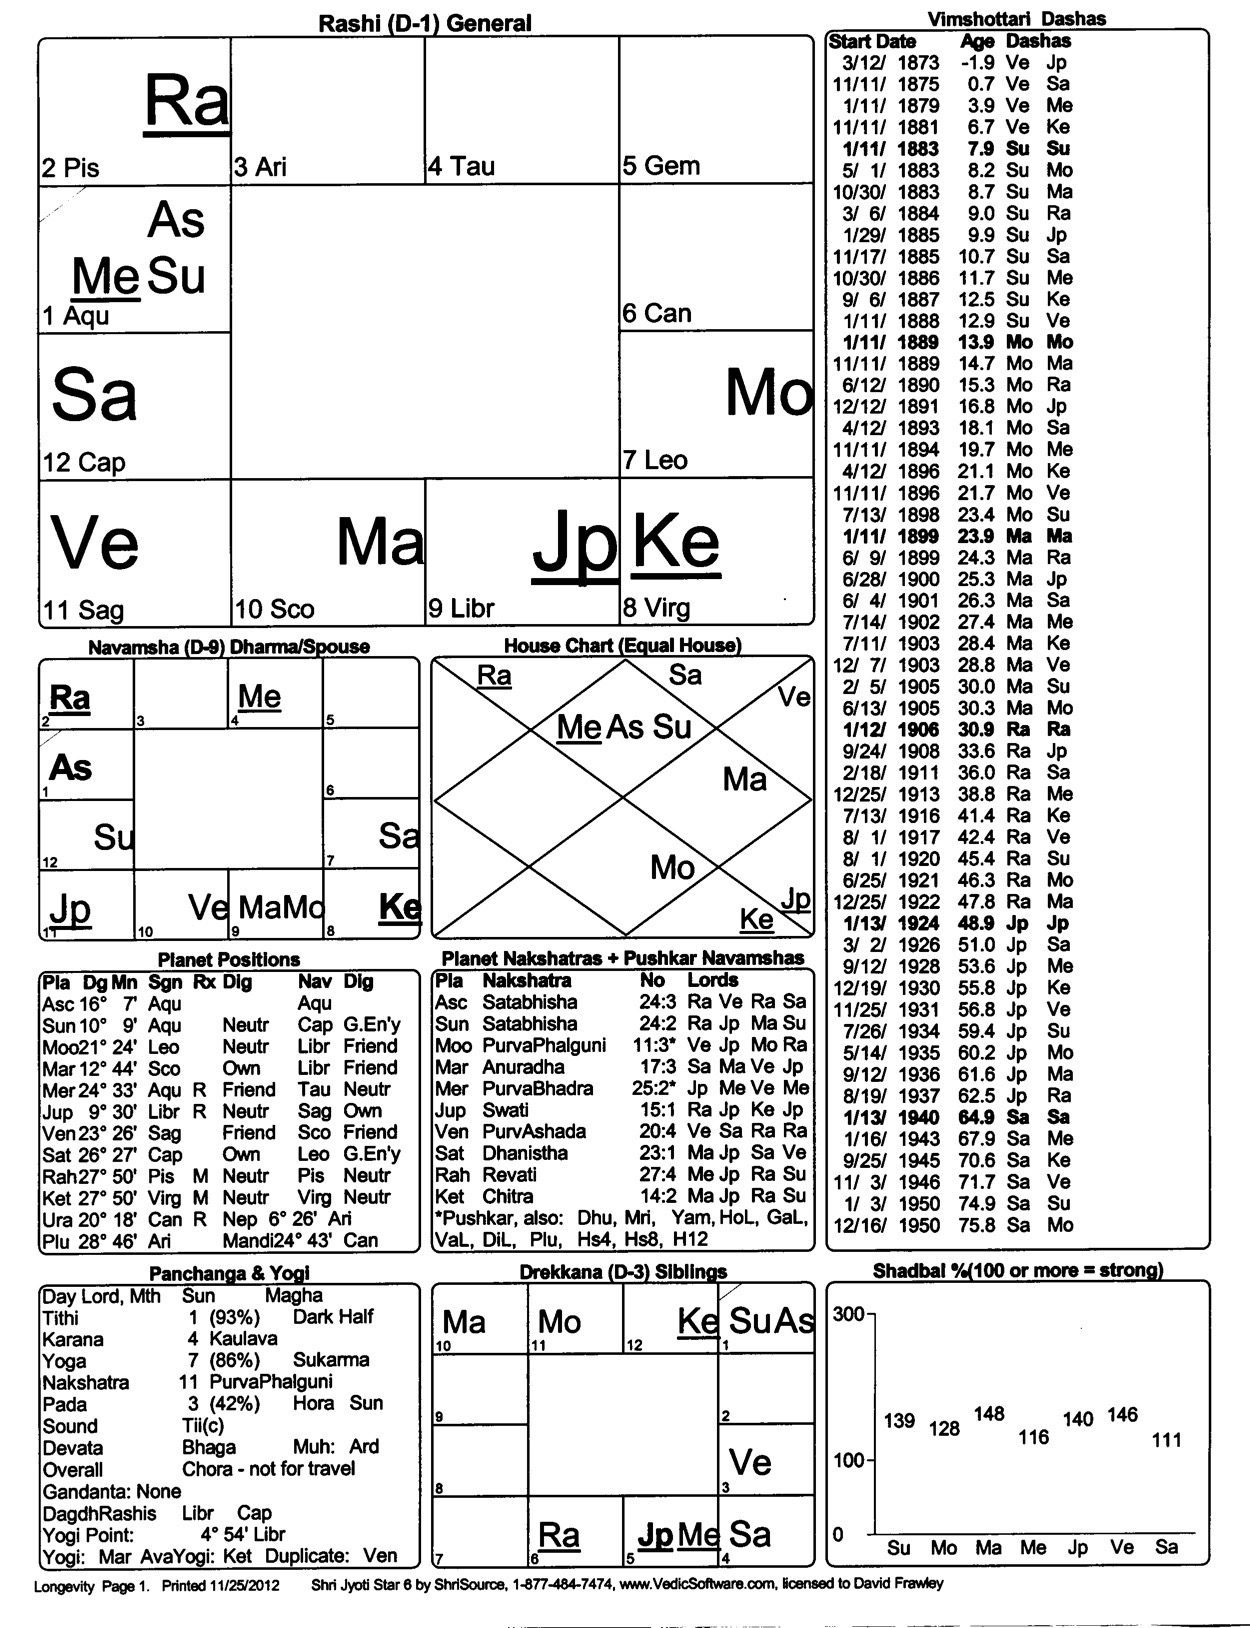
\includegraphics[width=10cm]{pics/Lesson6chart3.jpg}
\caption{}
\end{figure}


Whenever we are looking at charts of one type we should always try to look at charts of an opposite type in order to maintain a balanced view.

 

If we are looking at the charts of famous people we should also look at the charts of ordinary people. If we are looking at the charts of the wealthy, we should also examine the charts of those with financial difficulties. If we are looking at the charts of very spiritual people, we should balance this with the charts of the not so spiritual. If we are looking at charts of people who die young, we should balance this by looking at charts of people who live very long. That is what we will do in this instance.

 

This chart is of a woman who recently died at the rare old age of 121 years. She was quite active physically, taking up fencing at the age of 85, bicycling until the age of 100, and released a rap music record at the age of 121, just before her death. Her life style was not particularly healthy. She drank a lot of wine, ate lots of olive oil, chocolate and smoked cigarettes. She was hardly the example of a healthy life.

 



 

First let us examine the planetary periods at the time of birth to help determine her constitutional and congenital strength. Birth occurred in the very favorable period of Venus‑Jupiter‑Moon, three benefics, giving good congenital strength.

 

However, if we take a quick look at the chart it does not seem that good for longevity. The Ascendant Lord is in the difficult twelfth house. The eighth lord is retrograde in the Ascendant along with the seventh lord, the Sun, a Maraka. Jupiter, though in the ninth, is retrograde. Malefic Mars dominates the chart from the tenth house, exchanging signs with the Ascendant lord in the twelfth house, and aspecting the planets in the Ascendant. Malefic Ketu is in the eighth house of longevity. From the Moon Mercury, a Maraka for Leo, is located retrograde in the seventh house, another Maraka influence. Rahu is located in the eighth house from the Moon, another difficult position. Is the chart wrong we might think? However a deeper look reveals much more strength to the chart.

 

Saturn as the Ascendant lord in its own sign is a point of strength, though not in itself extraordinary. Most significantly the Moon is nearly full and in a good Nakshatra in the seventh house. The Moon as the sixth lord represents the immune system and resistance to disease. This strong Moon casts its effect upon the Ascendant and the planets within it. This gives a very strong immune system.

 

But the most important factor is the strength of Mars, which is very powerful with an extraordinary Ruchaka Yoga from all three major positions of the Ascendant, Sun and Moon. It is in the tenth, its best house, both from the Ascendant and the Sun. Mars aspects the Ascendant and exchanges signs with its lord, Saturn, putting its strong influence on both the Ascendant and its lord and therefore coloring the entire chart with its Yoga. Scorpio is also a fixed sign. This gives a powerful urge to live and express oneself. Mars is also the lord of the third house from the Ascendant, giving good vitality, interest in life and increasing longevity. Mars has benefics, Venus and Jupiter, on both sides fortifying it yet further.

 

Mars is the Yoga Karaka from the Moon, ruling the fourth and ninth from Leo, giving it yet more power. The strong Mars aspects the fourth from both Lagna and Moon providing a strong emotional resilience. Nothing could overcome her, make her afraid, intimidate her, disturb her or get her lost in sorrow. In short the strong Mars has aided her longevity rather than reducing it. This is one of the powers of a Mahapurusha Yoga. Yet for great longevity something more than this should be required. After all Mars is a reckless planet and a person under its influence is bound to take risks that must result in some harm. Hence there must be an element of great luck to compensate for the dangers of a strong Mars.

 

On top of this extraordinary Mars, Venus and Jupiter exchange signs in the eleventh and ninth houses affording the native such incredible good luck in life. This is a kind of Lakshmi Yoga, a combination that gives the abundance of Lakshmi, the Goddess of good fortune. Venus itself is the Yoga karaka for Aquarius and in the eleventh, a house of abundance, gives abundantly. The two planets are also lords of houses two and four from the Lagna, bestowing material comforts on the native as well as well. From the Moon sign, Venus and Jupiter exchange houses three and five, and are also lords of eight and ten. This benefic exchange of the third and eighth house lords, two houses of longevity, again boosts longevity. All the houses ruled by these two planets benefit by this exchange, strengthening many factors in the chart. This strong Jupiter in the ninth house in itself perhaps gives good paternal heredity.

 

The strength of Jupiter extends to Rahu, which is located in its sign Pisces. This boosts up the eighth from the Ascendant by aspect and the eighth from the Moon by location. Even Jupiters retrograde motion has some benefit. Retrograde planets aspect the previous house. Here Jupiter in the ninth aspects by being retrograde also the eighth house, boosting up its longevity potential. Even Mercury being retrograde adds some positive influence to Saturn, the Ascendant lord, which is located twelfth from it.

 

The fifth house both from Lagna and Moon is under strong influence of benefics Venus and Jupiter in several ways, both by aspects and by exchange, giving a happy mind and a lot of good karma from previous lives. It probably grants the good wishes of her children and a good relationship with them. The strong Moon in the seventh house gives a strong sexual vitality and interest in life as well. The Sun, Moon, Lagna, Mars and Mercury are all in fixed signs giving persistence and endurance. No planets are located in unfriendly signs.

 

If the Navamsha is correct the Lagna is vargottama and the chart has a powerful Raja Yoga of Venus and Mars exchanging signs as the ninth and tenth lords. However I have hesitated to go more into Navamsha because I have not the time to try to rectify it.

 

Death occurred in Venus‑Saturn‑Sun. Yoga Karaka planet, Lagna Lord, and Maraka. You cant live forever. I am not able to see why this period would be so bad by the rules of Vimshottari Dasha alone. That Venus has malefics around it, and that Saturn is second from Venus, may contribute to her demise. Sun is also seventh lord and seventh from the Moon, giving it Maraka powers.

 

Now the question obviously arises, why didnt any of the standard Maraka planets gain Maraka powers even after so many years? Clearly the chart was very strong, first by the position of Mars and second by the Venus-Jupiter exchange around it. Third the powerful Moon added its weight.

 

What I dont understand is why she survived Ketu Mahadasha. Ketu is in eighth from Lagna, and second, a Maraka house from Moon. Mercury must have been strong enough as Lord of Ketu to counter this.

 

Conclusion: The natives longevity was the result of very good heredity combined with lots of luck, and much enduring vital interest in life, a one in a million shot. She won the longevity lottery as it were. Her life-style was engaging but not particularly healthy. Only the factor of unusual luck could counter it. Hers is no example to emulate for those who wish to live long.

 

Could a good Vedic astrologer have predicted that this woman would live so long? Probably not, but a good astrologer should have been able to see that the person has a combination of tremendous drive plus a lot of luck.

 

Hence before you look at Maraka planets or even anything else try to see if there are other distinctive combinations in the chart to either support or deny it. Such distinctive features for good or ill may have the capacity to neutralize other less powerful factors. As usual we must start with a thorough analysis of the chart before jumping to dramatic conclusions.